%\documentclass[slideColor,pdf, fyma2]{prosper}
\documentclass[svgnames]{beamer}
\usepackage{beamerthemesplit}
\usepackage{tikz}
\usepackage{xcolor}
\usepackage{verbatim}
\setbeamertemplate{navigation symbols}{} % Vypnuti navigation baru
\usepackage[utf8]{inputenc}
\usepackage[czech]{babel}
\newcommand{\myuv}[1]{\quotedblbase #1\textquotedblleft}
\setbeamertemplate{footline}{\hskip52em\textbf{\texttt{\insertframenumber/\inserttotalframenumber}}\vskip1em}
\setbeamertemplate{headline}{}
\setbeamertemplate{caption}{\insertcaption}
\setbeamertemplate{caption label separator}{}
%\setbeamertemplate{footline}[frame number]

\begin{document}
\title{Efektivní algoritmy pro práci s~konečnými automaty}
\author{Martin Hruška\\{\small Vedoucí: Ing. Ondřej Lengál}}

\frame{\titlepage} 

\frame{\frametitle{Motivace}
		\textcolor{Green}{Motivace}
		\begin{itemize}
			\item Konečné automaty
				\begin{itemize}
					\item Široké spektrum použití -- překladače, zpracování přirozeného jazyka, návrh číslicových systému, \textcolor{red}{formální verifikace}
					\item Algoritmy pro \textcolor{red}{nedeterministické} konečné automaty, především \textcolor{red}{test inkluze}
				\end{itemize}
		\end{itemize}

		\textcolor{Green}{Cíl}
		\begin{itemize}
			\item Vytvořit knihovnu pro práci s~konečnými automaty
		\end{itemize}
}

\frame{\frametitle{Definice NKA}
	\textcolor{red}{Nedeterministický konečný automat (NKA)} je pětice $(Q,\Sigma,\delta,S,F)$, kde
	\begin{itemize}
		\item $Q$ je konečná množina stavů
		\item $\Sigma$ je vstupní abeceda
		\item $\delta$ je přechodová funkce $Q\times\Sigma\rightarrow 2^Q$
		\item $S\subseteq Q$ je množina vstupních stavů
		\item $F \subseteq Q$ je množina koncových stavů
	\end{itemize}

  \begin{figure}[htp]
    \begin{center}
      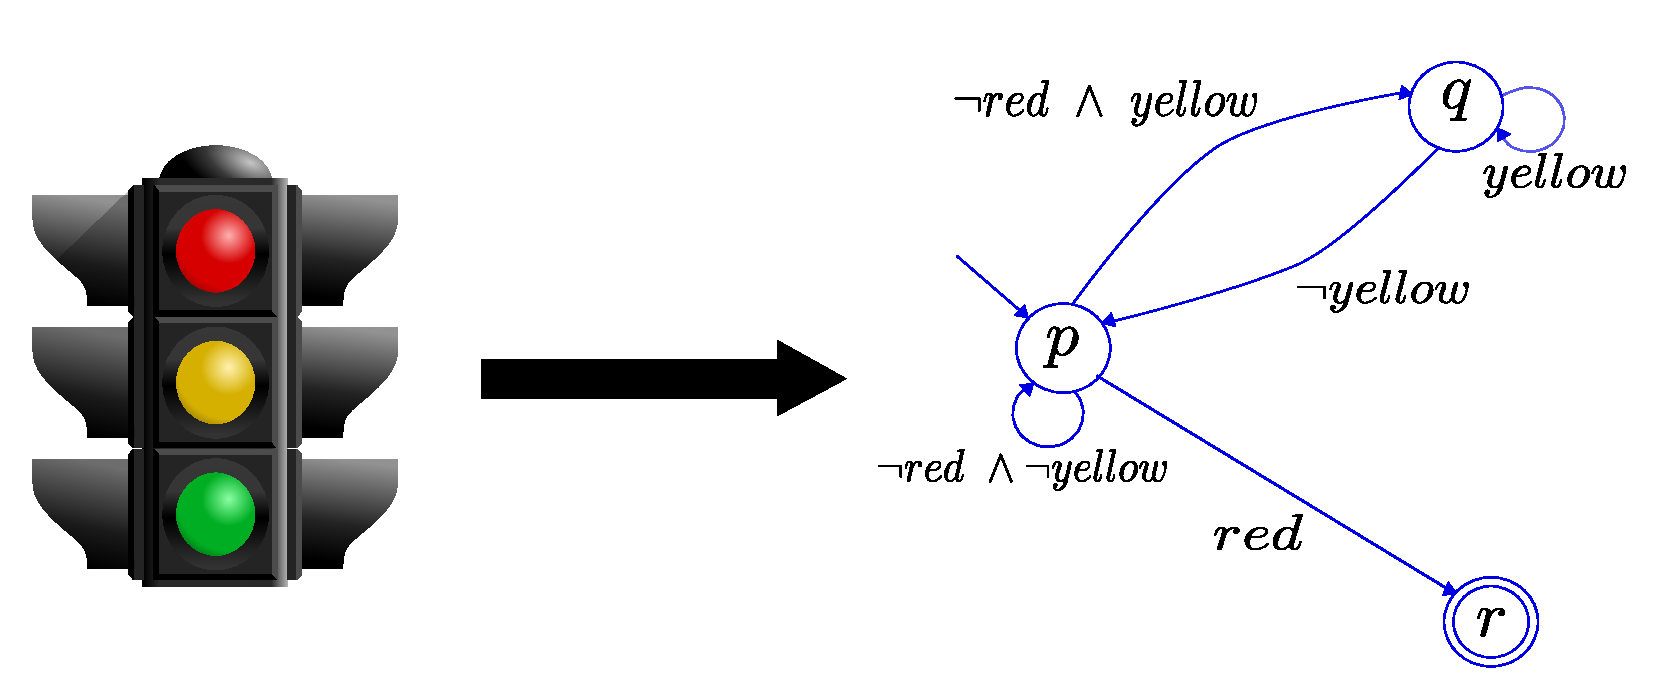
\includegraphics[scale=0.3]{tf_model.pdf}
    \end{center}
	\end{figure}
}


 \begin{comment}
		\begin{tikzpicture}[scale=0.09]
				\tikzstyle{every node}+=[inner sep=0pt]
				\draw [blue] (9.4,-29.6) circle (3);
				\draw (9.4,-29.6) node {$P$};
				\draw [blue] (29.9,-15.7) circle (3);
				\draw (29.9,-15.7) node {$Q$};
				\draw [blue] (29.9,-15.7) circle (2.4);
				\draw [blue] (33.8,-30.8) circle (3);
				\draw (33.8,-30.8) node {$R$};
				\draw [blue] (21.7,-50.3) circle (3);
				\draw (21.7,-50.3) node {$S$};
				\draw [blue] (21.7,-50.3) circle (2.4);
				\draw [blue] (51.1,-20.6) circle (3);
				\draw (51.1,-20.6) node {$T$};
				\draw [blue] (51.8,-41) circle (3);
				\draw (51.8,-41) node {$U$};
				\draw [blue] (51.8,-41) circle (2.4);
				\draw [blue] (3.2,-27.4) -- (6.57,-28.6);
				\fill [blue] (6.57,-28.6) -- (5.99,-27.86) -- (5.65,-28.8);
				\draw [blue] (11.88,-27.92) -- (27.42,-17.38);
				\fill [blue] (27.42,-17.38) -- (26.47,-17.42) -- (27.04,-18.25);
				\draw (20.6,-23.15) node [below] {$a$};
				\draw [blue] (10.93,-32.18) -- (20.17,-47.72);
				\fill [blue] (20.17,-47.72) -- (20.19,-46.78) -- (19.33,-47.29);
				\draw (14.9,-41.21) node [left] {$a$};
				\draw [blue] (12.4,-29.75) -- (30.8,-30.65);
				\fill [blue] (30.8,-30.65) -- (30.03,-30.11) -- (29.98,-31.11);
				\draw (21.33,-30.95) node [below] {$c$};
				\draw [blue] (32.82,-16.38) -- (48.18,-19.92);
				\fill [blue] (48.18,-19.92) -- (47.51,-19.26) -- (47.29,-20.23);
				\draw (39.8,-18.73) node [below] {$b$};
				\draw [blue] (36.38,-29.28) -- (48.52,-22.12);
				\fill [blue] (48.52,-22.12) -- (47.57,-22.1) -- (48.08,-22.96);
				\draw (43.5,-26.2) node [below] {$b$};
				\draw [blue] (36.41,-32.28) -- (49.19,-39.52);
				\fill [blue] (49.19,-39.52) -- (48.74,-38.69) -- (48.25,-39.56);
				\draw (41.85,-36.4) node [below] {$c$};
				\draw [blue] (48.93,-41.89) -- (24.57,-49.41);
				\fill [blue] (24.57,-49.41) -- (25.48,-49.66) -- (25.18,-48.7);
				\draw (35.85,-45.1) node [above] {$d$};
				\draw [blue] (32.22,-33.35) -- (23.28,-47.75);
				\fill [blue] (23.28,-47.75) -- (24.13,-47.33) -- (23.28,-46.81);
				\draw (27.12,-39.26) node [left] {$a$};
				\end{tikzpicture}
        \end{comment}



\frame{\frametitle{Algoritmy pro test jazykové inkluze}
		\textcolor{Green}{Klasický přístup}
		\begin{itemize}
			\item $L(A)\cap \overline{L(B)}=\emptyset$
			\item Nutná determinizace $\Rightarrow$ stavová exploze
		\end{itemize}

		\textcolor{Green}{Efektivní algoritmy}
		\begin{itemize}
			\item Umí pracovat s~nedeterministickými konečnými automaty
			\item	Nepotřebují vytvářet celý automat
			\begin{itemize}
				\item De Wulf, Doyen, Henzinger, Raskin. CAV'06.
				\item Abdulla, Chen, Holík, Mayr, Vojnar. TACAS'10.
				\item Bonchi, Pous. POPL'13.
			\end{itemize}
		\end{itemize}
	\begin{figure}[bht]
\begin{center}
	\scalebox{0.6}
	{
		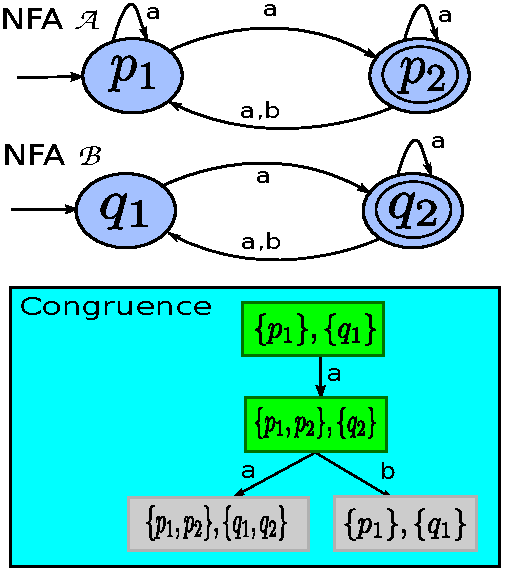
\includegraphics[scale=0.45]{congr1.pdf}
		\hspace{0.55cm}
  	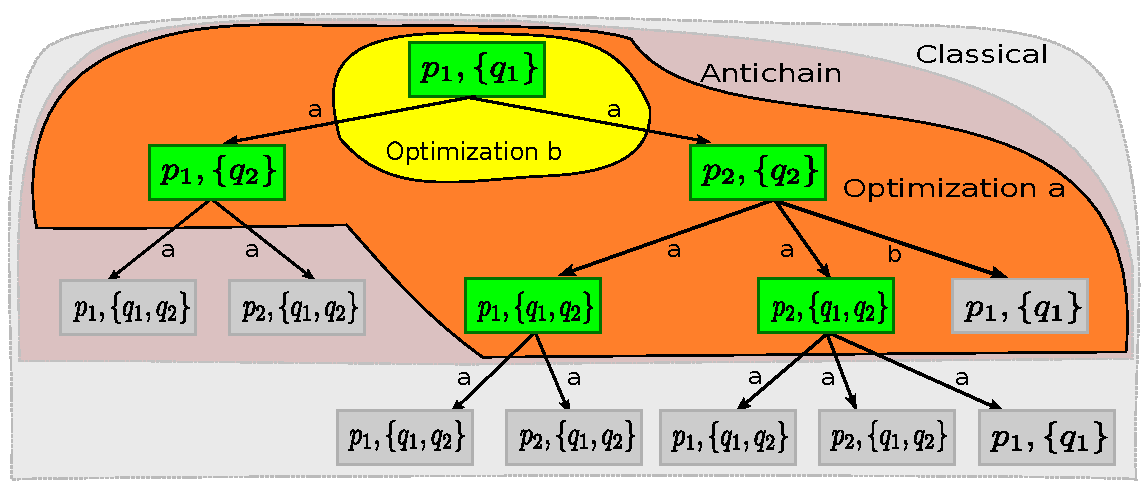
\includegraphics[scale=0.55]{ac1.pdf}
	}
  \label{automata}
\end{center}
\end{figure}	
}

\frame{\frametitle{Existující knihovny}
		\textcolor{Green}{dk.brics.automaton}
		\begin{itemize}
			\item balíček pro jazyk Java
			\item mutace \textcolor{red}{libfa} v~C a \textcolor{red}{fare} v~C\#
			\item pro test inkluze vyžaduje determinizaci
		\end{itemize}
		\textcolor{Green}{libgfsm, RWTH FSA Toolkit}
		\begin{itemize}
			\item starší knihovny v~C/C++
			\item opět problém s~nutností determinizace
		\end{itemize}
}			

\section{VATA}
\frame{\frametitle{VATA}
	\begin{itemize}
		\item Knihovna pro práci se \textcolor{red}{stromovými automaty}
		\item Zaměřena na oblast formální verifikace
		\item Podporuje explicitní a semi-symbolické kódování
		\item Cíl práce: rozšíření VATA pro \textcolor{red}{konečné automaty v~explicitním kódování}
	\end{itemize}
}

\section{Návrh}
\frame{\frametitle{Datové struktury}
  \begin{figure}[h]
  \begin{center}
  \minipage{0.5\textwidth}
  \begin{tikzpicture}
[
  scale=0.85,
  transform shape,
	gen/.style={thick,fill=gray!10},
	expl/.style={thick,fill=orange!50},
	bu/.style={thick,fill=green!40},
	td/.style={thick,fill=blue!30},
	other/.style={fill=yellow!10,dashed}
]

\node at(10,2) {Automata};

\node[expl,circle,draw] (aA) at(1.25,2) {\textit{$\mathcal{A}$}};
\node[expl,circle,draw] (aB) at(3.75,2) {\textit{$\mathcal{B}$}};
\node[expl,circle,draw] (aC) at(6.25,2) {\textit{$\mathcal{C}$}};


\node at(10,0) {\shortstack{Top-level\\ Lookup Tables}};

\node[minimum size=40pt](table1) at (2.75,-0.2) {};
\draw (2,0) rectangle +(0.5, .5) [td] node[midway] {\textit{$q_1$}};
\draw (2,-.5) rectangle +(0.5, .5) [td] node[midway] {};
\draw (2.5,0) rectangle +(0.5, .5) [td] node[midway] {\textit{$q_2$}};
\draw (2.5,-.5) rectangle +(0.5, .5) [td] node[midway] {};
\draw (3,0) rectangle +(0.5, .5) [td] node[midway] {\textit{$q_3$}};
\draw (3,-.5) rectangle +(0.5, .5) [td] node[midway] {};

\node[minimum size=40pt](table2) at (5,-0.2) {};
\draw (4.5,0) rectangle +(0.5, .5) [td] node[midway] {\textit{$q_1$}};
\draw (4.5,-.5) rectangle +(0.5, .5) [td] node[midway] {};
\draw (5,0) rectangle +(0.5, .5) [td] node[midway] {\textit{$q_2$}};
\draw (5,-.5) rectangle +(0.5, .5) [td] node[midway] {};


\draw[->,thick,dashed] (aA) -- (table1);
\draw[->,thick,dashed] (aB) -- (table2);
\draw[->,thick,dashed] (aC) -- (table2);


\node at(10.3,-2) {Transition Clusters};

\node[minimum size=35](cluster1) at (0.65,-2) {};
\draw (0.00,-2) rectangle +(1.25, .5) [td] node[midway] {\textit{$a$}};
\draw (0.00,-2.5) rectangle +(1.25, .5) [td] node[midway] {\textit{$\{q_1,q_2\}$}};
\draw (1.25,-2) rectangle +(1.25, .5) [td] node[midway] {\textit{$b$}};
\draw (1.25,-2.5) rectangle +(1.25, .5) [td] node[midway] {\textit{$\{q_1,q_2\}$}};

\node[minimum size=35pt](cluster2) at (3.55,-2.1) {};
\draw (2.75,-2) rectangle +(0.75, .5) [td] node[midway] {\textit{$c$}};
\draw (2.75,-2.5) rectangle +(0.75, .5) [td] node[midway] {\textit{$\{q_1\}$}};
\draw (3.5,-2) rectangle +(0.75, .5) [td] node[midway] {\textit{$e$}};
\draw (3.5,-2.5) rectangle +(0.75, .5) [td] node[midway] {\textit{$\{q_2\}$}};

\node[minimum size=35pt](cluster3) at (6.5,-1.75) {};
\draw (4.75,-2) rectangle +(1.25, .5) [td] node[midway] {\textit{$b$}};
\draw (4.75,-2.5) rectangle +(1.25, .5) [td] node[midway] {\textit{$\{q_2,q_2\}$}};
\draw (6.0,-2) rectangle +(1.25, .5) [td] node[midway] {\textit{$c$}};
\draw (6.0,-2.5) rectangle +(1.25, .5) [td] node[midway] {\textit{$\{q_2,q_3\}$}};

\node[minimum size=35pt](cluster4) at (8.5,-1.75) {};
\draw (7.5,-2) rectangle +(0.75, .5) [td] node[midway] {\textit{$e$}};
\draw (7.5,-2.5) rectangle +(0.75, .5) [td] node[midway] {\textit{$\{q_3\}$}};


\draw[thick,fill=black] (2.25,-0.25) circle (0.5mm);
\draw[->,thick,dashed] (2.25,-.25) -- (cluster2);

\draw[thick,fill=black] (2.75,-0.25) circle (0.5mm);
\draw[->,thick,dashed] (2.75,-.25) -- (cluster1);

\draw[thick,fill=black] (3.25,-0.25) circle (0.5mm);
\draw[->,thick,dashed] (3.25,-.25) -- (cluster3);

\draw[thick,fill=black] (4.75,-0.25) circle (0.5mm);
\draw[->,thick,dashed] (4.75,-.25) -- (cluster2);

\draw[thick,fill=black] (5.25,-0.25) circle (0.5mm);
\draw[->,thick,dashed] (5.25,-.25) -- (cluster4);
\end{tikzpicture}

  \endminipage
  \minipage{0.5\textwidth}
  \begin{tikzpicture}
[
  scale=0.85,
  transform shape,
	gen/.style={thick,fill=gray!10},
	expl/.style={thick,fill=orange!50},
	bu/.style={thick,fill=green!40},
	td/.style={thick,fill=blue!30},
	other/.style={fill=yellow!10,dashed}
]

\node at(10,2) {Automata};

\node[expl,circle,draw] (aA) at(1.25,2) {\textit{$A$}};
\node[expl,circle,draw] (aB) at(3.75,2) {\textit{$B$}};
\node[expl,circle,draw] (aC) at(6.25,2) {\textit{$C$}};


\node at(10,0) {\shortstack{Top-level\\ Lookup Tables}};

\node[minimum size=40pt](table1) at (2.75,0) {};
\draw (2,0) rectangle +(0.5, .5) [td] node[midway] {\textit{$q_1$}};
\draw (2,-.5) rectangle +(0.5, .5) [td] node[midway] {};
\draw (2.5,0) rectangle +(0.5, .5) [td] node[midway] {\textit{$q_2$}};
\draw (2.5,-.5) rectangle +(0.5, .5) [td] node[midway] {};
\draw (3,0) rectangle +(0.5, .5) [td] node[midway] {\textit{$q_3$}};
\draw (3,-.5) rectangle +(0.5, .5) [td] node[midway] {};

\node[minimum size=40pt](table2) at (5,0) {};
\draw (4.5,0) rectangle +(0.5, .5) [td] node[midway] {\textit{$q_1$}};
\draw (4.5,-.5) rectangle +(0.5, .5) [td] node[midway] {};
\draw (5,0) rectangle +(0.5, .5) [td] node[midway] {\textit{$q_2$}};
\draw (5,-.5) rectangle +(0.5, .5) [td] node[midway] {};


\draw[->,thick,dashed] (aA) -- (table1);
\draw[->,thick,dashed] (aB) -- (table2);
\draw[->,thick,dashed] (aC) -- (table2);


\node at(10,-2) {Transition Clusters};

\node[minimum size=35](cluster1) at (1.5,-2) {};
\draw (0.75,-2) rectangle +(0.5, .5) [td] node[midway] {\textit{$a$}};
\draw (0.75,-2.5) rectangle +(0.5, .5) [td] node[midway] {};
\draw (1.25,-2) rectangle +(0.5, .5) [td] node[midway] {\textit{$b$}};
\draw (1.25,-2.5) rectangle +(0.5, .5) [td] node[midway] {};

\node[minimum size=35pt](cluster2) at (3.25,-2) {};
\draw (2.75,-2) rectangle +(0.5, .5) [td] node[midway] {\textit{$c$}};
\draw (2.75,-2.5) rectangle +(0.5, .5) [td] node[midway] {};
\draw (3.25,-2) rectangle +(0.5, .5) [td] node[midway] {\textit{$e$}};
\draw (3.25,-2.5) rectangle +(0.5, .5) [td] node[midway] {};

\node[minimum size=35pt](cluster3) at (5.25,-2) {};
\draw (4.75,-2) rectangle +(0.5, .5) [td] node[midway] {\textit{$b$}};
\draw (4.75,-2.5) rectangle +(0.5, .5) [td] node[midway] {};
\draw (5.25,-2) rectangle +(0.5, .5) [td] node[midway] {\textit{$c$}};
\draw (5.25,-2.5) rectangle +(0.5, .5) [td] node[midway] {};

\node[minimum size=35pt](cluster4) at (6.5,-2) {};
\draw (6.25,-2) rectangle +(0.5, .5) [td] node[midway] {\textit{$e$}};
\draw (6.25,-2.5) rectangle +(0.5, .5) [td] node[midway] {};


\draw[thick,fill=black] (2.25,-0.25) circle (0.5mm);
\draw[->,thick,dashed] (2.25,-.25) -- (cluster2);

\draw[thick,fill=black] (2.75,-0.25) circle (0.5mm);
\draw[->,thick,dashed] (2.75,-.25) -- (cluster1);

\draw[thick,fill=black] (3.25,-0.25) circle (0.5mm);
\draw[->,thick,dashed] (3.25,-.25) -- (cluster3);

\draw[thick,fill=black] (4.75,-0.25) circle (0.5mm);
\draw[->,thick,dashed] (4.75,-.25) -- (cluster2);

\draw[thick,fill=black] (5.25,-0.25) circle (0.5mm);
\draw[->,thick,dashed] (5.25,-.25) -- (cluster4);


\node at(10,-3.75) {\shortstack{Sets of\\ Pointers to Tuples}};

\node[minimum size=25pt](set1) at (0.25,-3.75) {};
\draw (0,-4) rectangle +(0.5, .5) [td] node[midway] {};

\node[minimum size=25pt](set2) at (1.5,-3.75) {};
\draw (1,-4) rectangle +(0.5, .5) [td] node[midway] {};
\draw (1.5,-4) rectangle +(0.5, .5) [td] node[midway] {};

\node[minimum size=25pt](set3) at (2.75,-3.75) {};
\draw (2.5,-4) rectangle +(0.5, .5) [td] node[midway] {};

\node[minimum size=25pt](set4) at (3.75,-3.75) {};
\draw (3.5,-4) rectangle +(0.5, .5) [td] node[midway] {};

\node[minimum size=25pt](set5) at (4.75,-3.75) {};
\draw (4.5,-4) rectangle +(0.5, .5) [td] node[midway] {};

\node[minimum size=25pt](set6) at (6,-3.75) {};
\draw (5.5,-4) rectangle +(0.5, .5) [td] node[midway] {};
\draw (6,-4) rectangle +(0.5, .5) [td] node[midway] {};

\node[minimum size=25pt](set7) at (7.25,-3.75) {};
\draw (7,-4) rectangle +(0.5, .5) [td] node[midway] {};


\draw[thick,fill=black] (1,-2.25) circle (0.5mm);
\draw[->,thick,dashed] (1,-2.25) -- (set1);

\draw[thick,fill=black] (1.5,-2.25) circle (0.5mm);
\draw[->,thick,dashed] (1.5,-2.25) -- (set2);

\draw[thick,fill=black] (3,-2.25) circle (0.5mm);
\draw[->,thick,dashed] (3,-2.25) -- (set3);

\draw[thick,fill=black] (3.5,-2.25) circle (0.5mm);
\draw[->,thick,dashed] (3.5,-2.25) -- (set4);

\draw[thick,fill=black] (5,-2.25) circle (0.5mm);
\draw[->,thick,dashed] (5,-2.25) -- (set5);

\draw[thick,fill=black] (5.5,-2.25) circle (0.5mm);
\draw[->,thick,dashed] (5.5,-2.25) -- (set6);

\draw[thick,fill=black] (6.5,-2.25) circle (0.5mm);
\draw[->,thick,dashed] (6.5,-2.25) -- (set7);


\node at(10,-5.5) {Tuples of States};

\node(tup1) at (0.75,-5.5) {$(q_1, q_1)$};
\node(tup2) at (2.5,-5.5) {$(q_1, q_2)$};
\node(tup3) at (4.25,-5.5) {$(q_2, q_2)$};
\node(tup4) at (7,-5.5) {$(q_3, q_2)$};
\node(tup5) at (5.5,-5.5) {$()$};

\draw[thick,fill=black] (0.25,-3.75) circle (0.5mm);
\draw[->,thick,dashed] (0.25,-3.75) -- (tup1);

\draw[thick,fill=black] (1.25,-3.75) circle (0.5mm);
\draw[->,thick,dashed] (1.25,-3.75) -- (tup1);

\draw[thick,fill=black] (1.75,-3.75) circle (0.5mm);
\draw[->,thick,dashed] (1.75,-3.75) -- (tup2);

\draw[thick,fill=black] (2.75,-3.75) circle (0.5mm);
\draw[->,thick,dashed] (2.75,-3.75) -- (tup2);

\draw[thick,fill=black] (3.75,-3.75) circle (0.5mm);
\draw[->,thick,dashed] (3.75,-3.75) -- (tup5);

\draw[thick,fill=black] (4.75,-3.75) circle (0.5mm);
\draw[->,thick,dashed] (4.75,-3.75) -- (tup2);

\draw[thick,fill=black] (5.75,-3.75) circle (0.5mm);
\draw[->,thick,dashed] (5.75,-3.75) -- (tup3);

\draw[thick,fill=black] (6.25,-3.75) circle (0.5mm);
\draw[->,thick,dashed] (6.25,-3.75) -- (tup4);

\draw[thick,fill=black] (7.25,-3.75) circle (0.5mm);
\draw[->,thick,dashed] (7.25,-3.75) -- (tup5);


\end{tikzpicture}

  \endminipage
  \caption{Datová struktura pro ukládní přechodů \textcolor{red}{konečných (vlevo)} a \textcolor{green}{stromových (vpravo)} automatů}
  \end{center}
  \end{figure}
}

\section{Použité algoritmy a optimalizace}
\frame{\frametitle{Použité algoritmy}
  \begin{itemize}
    \item Použit a testován algoritmus fungující na základě výpočtu kongruenčního uzávěru množiny stavů
    \item Optimalizován speciálně na test inkluze
    \item Použity implementační optimalizace (cachování již spočtených množin)
  \end{itemize}
}

\section{Evaluace}
\frame{\frametitle{Porovnání s~OCaml verzí}

  \begin{center}
  \begin{figure}
    \includegraphics[scale=0.35]{plot_hkc.png}
  \end{figure}
  \vspace{0.5cm}
   \begin{tabular}{ | l | r | r |}
   \hline
    & \textbf{OCaml} & \textbf{VATA} \\ \hline \hline
    rychlejší & $26\%$ & $74\%$ \\ \hline
   \end{tabular}
 \end{center}
}
\frame{\frametitle{Porovnání s~VATA pro TA}

  \begin{center}
   \begin{tabular}{ | l | r | r |}
   \hline
    & \textbf{OCaml} & \textbf{VATA} \\ \hline \hline
    vítěz & $75\%$ & $25\%$ \\ \hline
   \end{tabular}
 \end{center}
} 

\section{Možnost dalšího vývoje}
\frame{\frametitle{Další vývoj}
  \begin{itemize}
    \item Optimalizace algoritmu používajícího principu antichainů
    \item Využití simulace
  \end{itemize}
}

\section{Závěr}
\frame{\frametitle{Závěr}
  tady budou znovy vysledky
}
\end{document}
